\documentclass[10pt]{article}

\usepackage{spheric}
%%%TITLE
\title{Study on Dynamic Behaviors of Liquid-filled Flexible Multibody Systems under the Low-gravity Environment}
\date{}

%%AFFILIATIONS
\author[$\relax$]{Weizhen Kong$^\dagger$}

\affil[$\relax$]{Beijing Institute of Technology, China}

\author[$\relax$]{Qiang Tian}

\affil[$\relax$]{\href{mailto:weizhen_kong@aliyun.com}{weizhen\_kong@aliyun.com}}





%%DOCUMENT
\begin{document}

\maketitle

%\SelectedTopics{}

%%PLEASE PUT YOUR ABSTRACT HERE
\begin{abstract}
There are vast kinds of liquid-filled flexible multibody systems in engineering fields, especially the aerospace field. In early studies, the coupled dynamic behaviors of the liquid-filled flexible multibody systems were mainly studied by using equivalent methods, in which the liquid is generally simplified as a rigid body system consisting of some lumped masses with springs or some pendulums, both representing the main slosh modes. However, these approaches are not able to reflect the liquid splashing phenomenon. A computation method is used to study the coupled dynamics of a partially liquid-filled flexible multibody system, where the liquid is modeled by using SPH method and the flexible bodies are described by using the Absolute Nodal Coordinate Formulation (ANCF). The fluid behavior is quite different in the absence of gravity since the inertia force is not the dominant force. The CSF model is used to introduce the surface tension force into the momentum equation.

A simulation is presented: a liquid-filled spacecraft with flexible manipulator arms grabbing a liquid-filled container. As shown in Figure 1, all the flexible components are described by element of ANCF and all rigid bodies in the system are modeled via the Natural Coordinates Formulations (NCF), like the mechanical claw and the handle connected to the container. SPH particles are used to describe the liquid and virtual particles are introduced for the coupling between finite elements of ANCF and particles of SPH.
\begin{figure}[!htb]
\centering
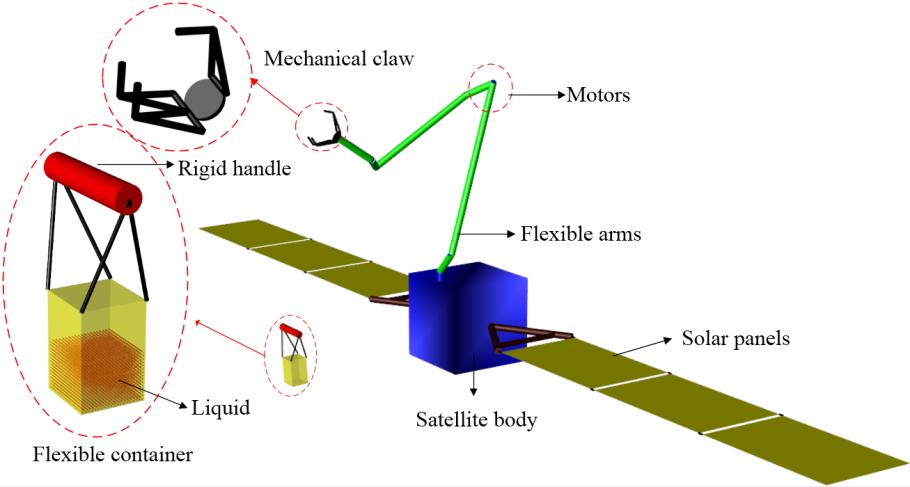
\includegraphics[width=0.9\textwidth]{38-1.png}
\caption{Liquid-filled spacecraft with flexible arms}\label{fig:38}
\end{figure}

\end{abstract}


%%THE END OF ABSTRACT

%\addbib

\end{document}
